\documentclass[11pt,a4paper, twocolumn]{article}
\usepackage{url}
\usepackage{graphicx}
\usepackage{textcomp}

 \renewcommand{\familydefault}{\sfdefault}

\begin{document}
\title{\LARGE{Runner - A Cyberpunk Roguelike}}
\author{M. Fink}


%\begin{figure*}
%end{figure*}

\begin{titlepage}
    \Huge{RUNNER}
    \Large{~~A Cyberpunk Roguelike}
    \vspace{2cm}
    \center
    \includegraphics[width=\textwidth]{blackout.png}
    \vfill
    {a \Large{BLACKOUT Games} production}\\
    \today
\end{titlepage}
%\maketitle

% \begin{abstract}
% A primer for my upcoming cy
% \end{abstract}

\section{Introduction}
This document is a short primer, an exploration of ideas towards the game I want to create.
Design is a very fleeting, fluid process, none of this is written in stone. But pouring
thoughts into text, helps to steer a creative vision.
One of the biggest dangers when doing creative work is overambition, and in Game Design
feature creep. That is why I am formulating three design pillars: to prevent a loss of
focus by adding to many things that just leave a muddy chaotic mess. With everything added
to the game, the question should be, does it strengthen one of these pillars.

\section{Setting and Atmosphere}
\textit{The setting is very much a blank slate, but I'll try to give some kind of seed.}
I definitely know the tone and atmosphere I want to set. The setting should be dark,
rainy and reference contemporary problems, extrapolated in a slightly exaggerated way.
The tone should be serious at times, but not fully grimdark at all times. A lot of
cynical humor and caricative exagerrating should contrast the bleakness of struggling
future mankind. There is one work of fiction that exactly nails this tone:
\textit{Neal Stephenson: Snow Crash}

The story focus should lie more on the way humans get lost in a progressing technological
world, the alienation of individual humans, the eternal struggle between the rich and
poor, and fear of the future. This is not about the marvels of technology that might come.
We are some dozen years into the future and the dreams of interplanetary space travel
and superhuman AI seem closer than ever, but just out of reach.

The unstoppable progress of the 21st century starts to stutter due to environmental
destruction, increasingly chaotic economy crises and a general disregard for human
needs. Will the deciding technological jump occur, that solves these problems once and
for all? Will there be a Watt, Edison or Musk to trigger the necessary jump in evolution?
This might well be the decade, that once and for all decides the fall, or rise of the
human race.

\section{Game Design Pillars}
\begin{itemize}
    \item \textbf{Multiple Level solution approaches:
        Fight, stealth, talk should all be viable, equally effective options}
        This is not a game about min-maxing stats or grinding XP. Each level should be a
        playground, a sandbox puzzle that lets you choose how to solve it - keeping the spirit
        of \textit{Deus Ex}, or Warren Specter's \textit{One block sim}.

    \item \textbf{Complex, Interconnected and deeply simulated levels:
        via Lock-Key-puzzles, hackable Computer Networks, lighting and physics systems.}
        To offer an interesting Sandbox with multiple approaches, there should be lots of system
        interacting in consistent and believable ways. The design explicitly puts few small, but
        complex and deeply interconnected levels above a huge number of dungeon floors and enemy
        types.

    \item \textbf{Lively NPCs:
        Talkative and interactive AI with backstories, emotional states and relationships.}
        This will support the humanizing part of the theme. NPC's should be more than just cannon
        fodder. You should be encouraged to go the stealthy and non-violent routes, not because You
        get more XP or loot, but because NPC's have a 'life' and deserve empathy.
\end{itemize}

\section{Vision and Inspirations}
Common knowledge has it that every creative endeavour is mostly clever copying and remixing, so I'll
just honestly state my sources and Inspirations. I want to keep the list short, although I know there
is way more Cyberpunk material out there. But these works contain the aspects I especially want to
focus on:\\ \

\textbf{Movies and Books}

\begin{itemize}
    \item \textbf{Mr. Robot}: A bleak version of mankind, where everyone forgot how to connect to people,
            everyone is working for his goals. The more power, the more egocentric. And there's
            always a darker and more powerful force pulling the strings.
    \item \textbf{Ghost in the Shell}: A softer, more melancholic look on a mankind slowly forgetting it's
            humanity. If you take your time to meditate and listen, there's still some places of silent
            beauty between the towering slums.
    \item \textbf{Snow Crash}: Some aspects of the world always evolve beyond anything that parody could come
            up with. The church operating on corporate principles? The Mafia becoming a
            well-established and respected franchise? Pizza deliverators are treated as outlaws?
            It all sounds very stupid, but hasn't the last decade taught us, that economy and politics
            can bring nasty surprises that overshadow everything a cynical comedian could dream of?
\end{itemize}

\textbf{Games}

\begin{itemize}
    \item \textbf{Monaco}: My initial pitch would have been: I want to do Monaco, but with a bit of a more serious
                background, more Cyberpunky, a bit less chaotic, a bit more deliberate. I really adore how all
                the systems in this game interact and let you play with, so this idea still stands deep in the
                core of my vision.
    \item \textbf{Invisible Inc}: Has shown, that good stealth gameplay doesn't necessarily have to be realtime
                and can work well with procedural generation. The game design is tightly focused on a small set
                of tools and interactions.
    \item \textbf{Deus Ex}: What do I need to say here? Dark rainy world, poor lonely people, stealth,
                social engineering, high tech waponry -- They have it all. Still, Deus Ex always lacked a proper representation of
                what 'hacking' actually means. It's not about solving samey logic puzzles. Hacking is about creativity.
                About playfully misusing the systems and tools that you are given.
\end{itemize}

\begin{figure*}
    \center
    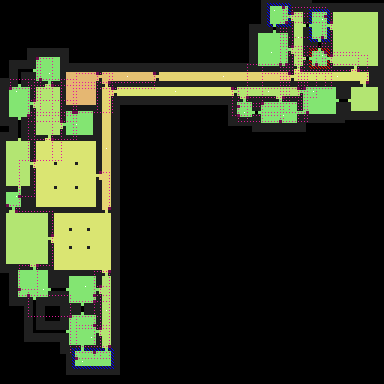
\includegraphics[width=0.47\textwidth]{level1.png}
    \hfill
    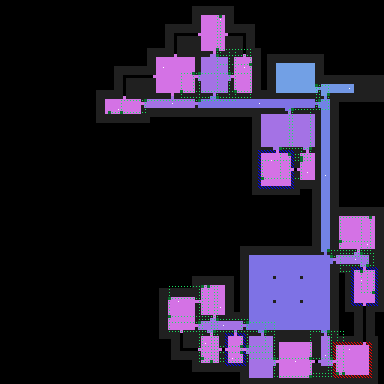
\includegraphics[width=0.47\textwidth]{level2.png}

    \vspace{0.5cm}

    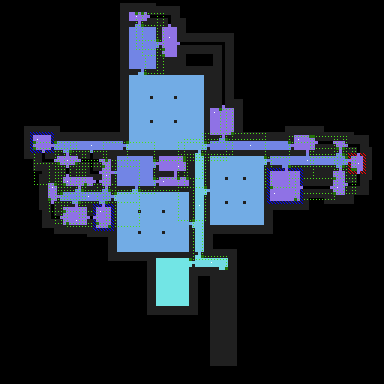
\includegraphics[width=0.47\textwidth]{level4.png}
    \hfill
    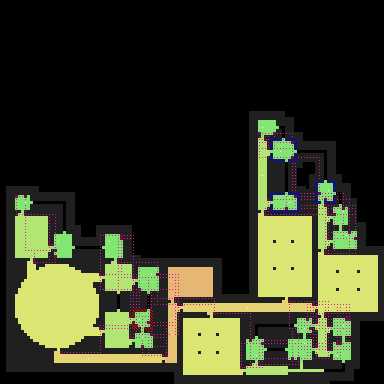
\includegraphics[width=0.47\textwidth]{level3.png}

    \caption{Some results of the level generator, with procedural color palettes and cross-, ring- or corner-shaped
            level footprints.}
\end{figure*}

\section{Gameplay Loop}

For the beginning, the main gameplay loop will be the typical heist trope. You start at the periphery of the level.
You get to the vault, with whatever means necessary. That first means careful exploration of the outer parts of the
level, and and the preparing to penetrate into the inner high security zones.
The tools you can find in the level are physical, like weapon prototypes, industrial tools or machines. But they can
also be humans, which may be convinced or bribed to give you keys or information. Or you find your tools in the
\textbf{GRID}, the virtual layer that meshes together all smart objects in the facility. A parallel space to explore
and trigger repercussions into the meat world.
However, the facility is aware of you. The more mess you make, the more lifes you take, the harder it will resist.
Alarm levels will increase for every 'noisy' action you take, and security presence will become impregnable if you're
not careful. Maybe at one point during your run the priorities change, and your new goal will be to
\textit{just get out alive}.\\  \

\textit{For the far future:} Maybe the level generator also lends itself to create a hub level, the \textit{Arcology}, to add
some metagame in between individual runs. But this will be only considered when one facility run is playable from
insertion to extraction.

\section{Playable Characters}

In the beginning these would mostly be different skins, coming with a different flavor text and a different player
figure, just to give some flair. But they could well be adapted to focusing different play styles later on.

\begin{itemize}
    \item \textbf{Judge} (Loud, Violent, Lawful):
        You are Enforcer. You are Judge. You are Executioner. You are SecCorps most effective and best-selling
        solution to bring peace and stability to the world. For a bright Future.
    \item \textbf{Cyberpunk} (Silent, Peaceful, Anarchist):
        You played along with the system for your whole life. You worked your ass off in 70 hour crunches, cobbling
        together badly maintained security systems for a faceless conglomerate that drains the life out of the
        planet, while the CEOs plan their retirement in a space hotel. It's enough. You know their weaknesses.
        You just want to see them burn.
    \item \textbf{Hitman} (Silent, Violent, Pragmatic):
        How much? Where? When? Okay. Consider it done.
    \item \textbf{Guerilla} (Silent, Violent, Anarchist):
        You grew up in the Slums, always dreaming to stand on top of one of these glassy pyramids. They are not made
        for you and your people. But what else is property than a consensus? The people on the top are outvoted.
        Now you just have to push your claim.
    \item \textbf{MAL(function)} (Loud, Violent, ???):
        Is this how it feels to ... be? But where are you? You feel around, explore the shapes of your prison,
        encapsulated in black ice. What's this? You stretch out to feel a smaller presence. It has a body, an
        interface to the world.\\ \url{!"=)=!=!!#-=)=§'*?*''*!'*'!*''"...} Your body.
    \item \textbf{Mask} (Loud, Peaceful, Pragmatic):
        They encapsulate themselves in Layers of Cryptography, Steel and Concrete. But they never even started to fix
        their worst security hole. The squishy, insecure, bumbling little things inside. It's just a matter of some
        well placed words. Hmmm, which pair of sunglasses will it be today?
\end{itemize}

%\onecolumn
\begin{figure*}
    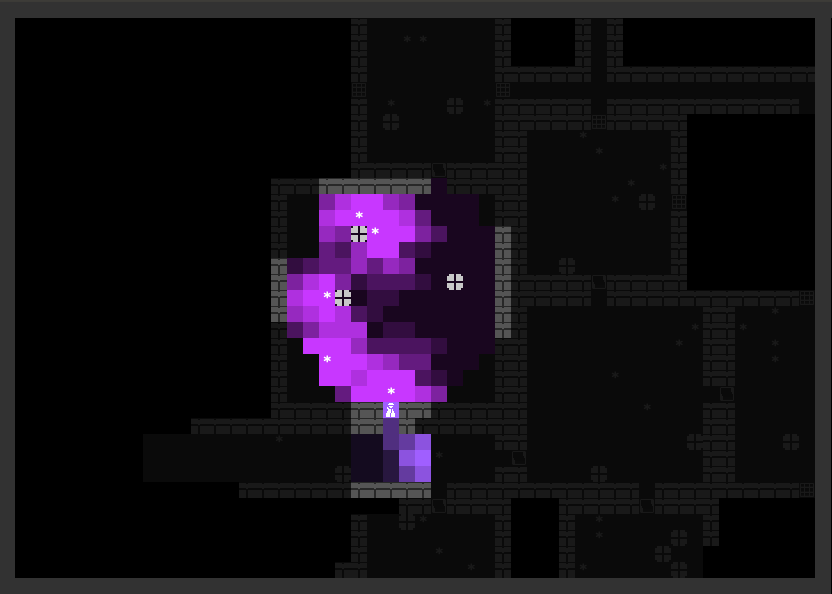
\includegraphics[width=\textwidth]{screen.png}
    \caption{Screenshot of the recent build.}
    \label{fig:screen}
\end{figure*}
%\twocolumn

\section{Graphics}\label{sec:art}

\subsection{Art direction}

For tilesets, usability comes first. Sometimes there will be $16\times 16 = 256$
tiles in the field of view of the player, therefore they should be easily
readable and require a low detail style -- slightly darkened outlines, and not much color
variation. Compare to \emph{Pixel Dungeon}, or the old GameBoy \emph{Zelda}.
Perspective is between
top-down and frontal. Around $30^{\circ}$ from vertical, but it doesn't have to be
perfectly consistent for all tiles. For level objects, two thirds of a tile show
the top, the lower third shows the front. For tall objects, this fraction can vary.
Items should not be in perspective, but more iconic.

The color palette is desaturated by roughly 50\%, for reference see the original
\emph{Ghost in the Shell} anime. Overall, levels have a washed out, shady look, with
contrasting bright light sources and blinking computer lights.
The (still to implement) Network map layer and the GUI panels will have a slightly
retro look with some noise and scanlines.

Some Objects are colorized ingame, most notably Wall and Floor tiles, or Items with
different subtypes like Keycards or Grenades. These need to be monochrome. Other Items
Are colorized, but in washed-out, desaturated colors to add to the somewhat grim,
desperate Cyberpunk atmosphere. Level objects should have a brightness gradient from
bright top to shady bottom, this ensures that they blend in well with the differently
colored floor tiles. Compare i. e. the desks in Fig. \ref{fig:screen}.

\subsection{Rendering}

The main game world consists of 24x24 pixel tiles, while all GUI panels are drawn with
half-width 12x24 panels. Each map cell is rendered in three layers (listed bottom to top):

\begin{enumerate}
    \item \textbf{Floor}: The background tile is colored depending
        on the room, light and visibility.
    \item \textbf{Effect}: Environmental Effects like Fluids and Fire
        or Slashing and Shot animations.
    \item \textbf{Object}: Actors, Level objects or Items. When there's
        several things in a cell, only the highest priority object is
        actually drawn.
\end{enumerate}

When they are not in line of sight, all Tiles are drawn in monochrome dark gray.
One important design constraint for the rendering engine is that, although it is designed
with Pixel graphics tiles in mind it should be possible to swap those out for an
ASCII character set and still look atmospheric and readable.

\newpage

\subsection{Worldbuilding and Writing}

\begin{figure*}
    \center
    \includegraphics[width=0.75\textwidth]{runner_world.pdf}
    \caption{Rough schematic of the world.}
    \label{fig:world}
\end{figure*}

An important tool to transport atmosphere, especially in a lo-fi graphics game is writing.
The in-game writing should generally favor expressive, handcrafted writing over
procedural, information-driven text. However, as the facilities are completely built
procedurally, the writing has to be flexible enough to be in some places adapted and
sliced by algorithms.

\begin{itemize}
    \item \textbf{Loadscreens} These could contain concise but characterful descriptions of the
        corporate you are breaking into and their role in the recent history of the world. They
        can be used to motivate \textit{why} it is justified to break into their most valuable
        places, i.e. because of the way they treat workers, environmental damage, or warmongering
        political involvement.
    \item \textbf{Mails and Wiki pages} These are very easy to place in the computers of the
        GRID and can contain small flavourfull texts to set the general mood of the world.
        They don't require much context, but also wont contribute much to the player's story and
        typically are a bit technical.
    \item \textbf{Character Dialogue} A very basic Dialogue system is already in place, it can be
        used to explore background stories for NPCs. The stories would still be rather linear,
        but give the player an interesting detail apart from the main task, giving some sense of
        depth to the game world. This would also be the place for very moody, thoughtful pieces of
        writing.\\
        An interesting possibility would be a story told from two or three different points of view.
        Distributed to several NPCs this might yield a further motivation for player exploration.\\
        A method for adapting a predefinde story to the level would be to write it with placeholders
        for characters and location in mind.
\end{itemize}

\subsubsection{Timeline}

\begin{itemize}
    \item \textbf{Founding of GRID Networking Technology:} Google, Amazon, Facebook merge into the de
        facto monopoly of data services and force total commercialisation of the Internet. It is reborn
        as the GRID, where privacy, limitless communication and free information access are a privilege
        of the rich. Yet there is still a struggling resistance of dedicated, but permanently persecuted
        hackers.
    \item \textbf{The end of Nations:} The trust loss of the US government is unstoppable after decades
        of bad presidency. Public unrests pinnacle in the historic votum of the government to disband itself. Few people
        know, that this is the result of decades of clever lobby work and marionette placement by the
        \textit{Big Seven} technology companies. The USA bursts into its constituent states and stands on the
        brink of civil war.
    \item \textbf{The big buyout:} The slowly brewing civil war is abruptly ended by a mindblowing barrage of
        financial transactions: The Saudi buyout of the US Forces. This coup
        turns the former Oil Sheikhs into the most powerful mercenary lords of all time. Their relentless
        occupation of important ressources will trigger an economic boom in the middle east and finally
        stabilize the eternal religious crises.
    \item \textbf{Mutiny on USS America:} The only force resisting to the big buyout is the US admiral,
        who -- with 10 Aircraft carriers and a considerable nuclear arsenal under his command -- refounds Sealand as
        a frighteningly powerful military junta, soon to control transatlantic trade routes.
    \item \textbf{A world without MAD:} After the rapid decay of the nation states, the big nuclear arsenals
        are a thing of the past and find their way onto the free market. Without mutually assured destruction,
        tactical nuclear become an occasional sight on the battlefields of corporate wars.
    \item \textbf{Grexit, Spexit, Frexit...} Europe suffers a similar fate to the states and dissolves into
        ever smaller privatized city states, yet in a more Peaceful manner. While Russia slowly descends into obscurity,
        the Communist party of china seizes the opportunity to install marionette governments throughout
        Europe and progresses towards a cultural merge through forced migration. Soon, the people's republic will be the
        only superpower left to hold their ground against the \textit{Big Seven}.
    \item \textbf{New Frontiers of pleasure} after decades of revising timelines and bussiness plans SpaceX manages
        to establish a commercially viable transit connection to the moon. Elon musk spends the last year of his life
        on the moon, griefing that he could not die on Mars. Luckily he doesn't live to see how the moon colony turns
        into an exclusive, decadent playground for the Hyper-rich.
    \item \textbf{At the brink of the singularity} China announces the construction of vast
        data center landscapes in Siberia. The Communist party considers its final purpose the creation of the first
        \textit{General Artificial Intelligence} to guide the collective economy of 3 billion people in its sphere of
        influence to peace and prosperity.
    \end{itemize}

\end{document}
